\section{Canopy Analysis}

Canopy analysis converts captured RGB images into quantitative plant traits.
The main output is canopy area over time, which can be used to quantify plant
growth dynamics. The analysis pipeline also generates diagnostic figures that
allow users to evaluate whether plant segmentation was successful. Correct
segmentation is the most important step in the analysis. Therefore, users
should first tune segmentation settings on a few representative images before
processing a complete experiment. The main output of this pipeline is a file
\texttt{combined\_traits.csv} which contains all derived plant measurements for
each individual plant in one or more images.

\subsection{Input Images}

The canopy analysis pipeline operates on timestamped images produced by the
Phenopi acquisition system. By default, these images are stored in:

\begin{verbatim}
$PHENOPI_ROOT/captures
\end{verbatim}

Image filenames should follow the standard capture format:

\begin{verbatim}
capture_YYYYMMDD_HHMMSS.jpg
\end{verbatim}

\subsection{Running Canopy Analysis}

The analysis is executed from the Phenopi repository directory using the canopy
analysis command line interface:

\begin{verbatim}
python -m scripts.analysis.analyze_canopy \
  --input data/images \
  --output results \
  --rows 5 \
  --columns 8 \
  --threshold 120 \
  --fill-size 200
\end{verbatim}

Available options can be displayed with:

\begin{verbatim}
python -m scripts.analysis.analyze_canopy --help
\end{verbatim}

The most important user-defined parameters are the color channel used for
segmentation, the threshold value, and the minimum object size retained after
segmentation.

\subsection{Selecting a Color Channel}

Phenopi relies on PlantCV to separate plant tissue from the background by
thresholding one channel from a selected color space. Different channels
emphasize different image properties. For example, some channels primarily
describe brightness, while others describe differences in color. Before running
the full analysis, users should inspect the color-space diagnostic output
(\autoref{fig:color-space-selection}). The best channel for separation is
usually the one where plants appear clearly different from all non-plant
objects. The goal is not to create a visually attractive image, but to maximize
contrast between the two classes: plant and background.

\begin{figure}[ht]
    \centering
    \includegraphics[width=\textwidth]{images/color_space_debug.png}
    \caption{
    Example color-space diagnostic image. Each panel shows the same image after
    conversion to a different color channel. A suitable channel should maximize
    the difference between plants and the surrounding tray, soil, and pot
    material.
    }%
    \label{fig:color-space-selection}
\end{figure}


\subsection{Selecting the Threshold Value}

After selecting a color channel, the pixel intensity histogram should be
inspected. The histogram shows how common each pixel intensity value is in the
selected channel. Pixels on one side of the threshold are classified as plant
tissue, while pixels on the other side are removed as background. A threshold
that is too low may include soil, algae, shadows, or pot edges. A threshold
that is too high may remove darker leaves and underestimate canopy area. In the
provided example histogram (\autoref{fig:threshold-histogram}), a value around
$\numrange{140}{145}$ would be appropriate.

\begin{figure}[ht!]
    \centering
    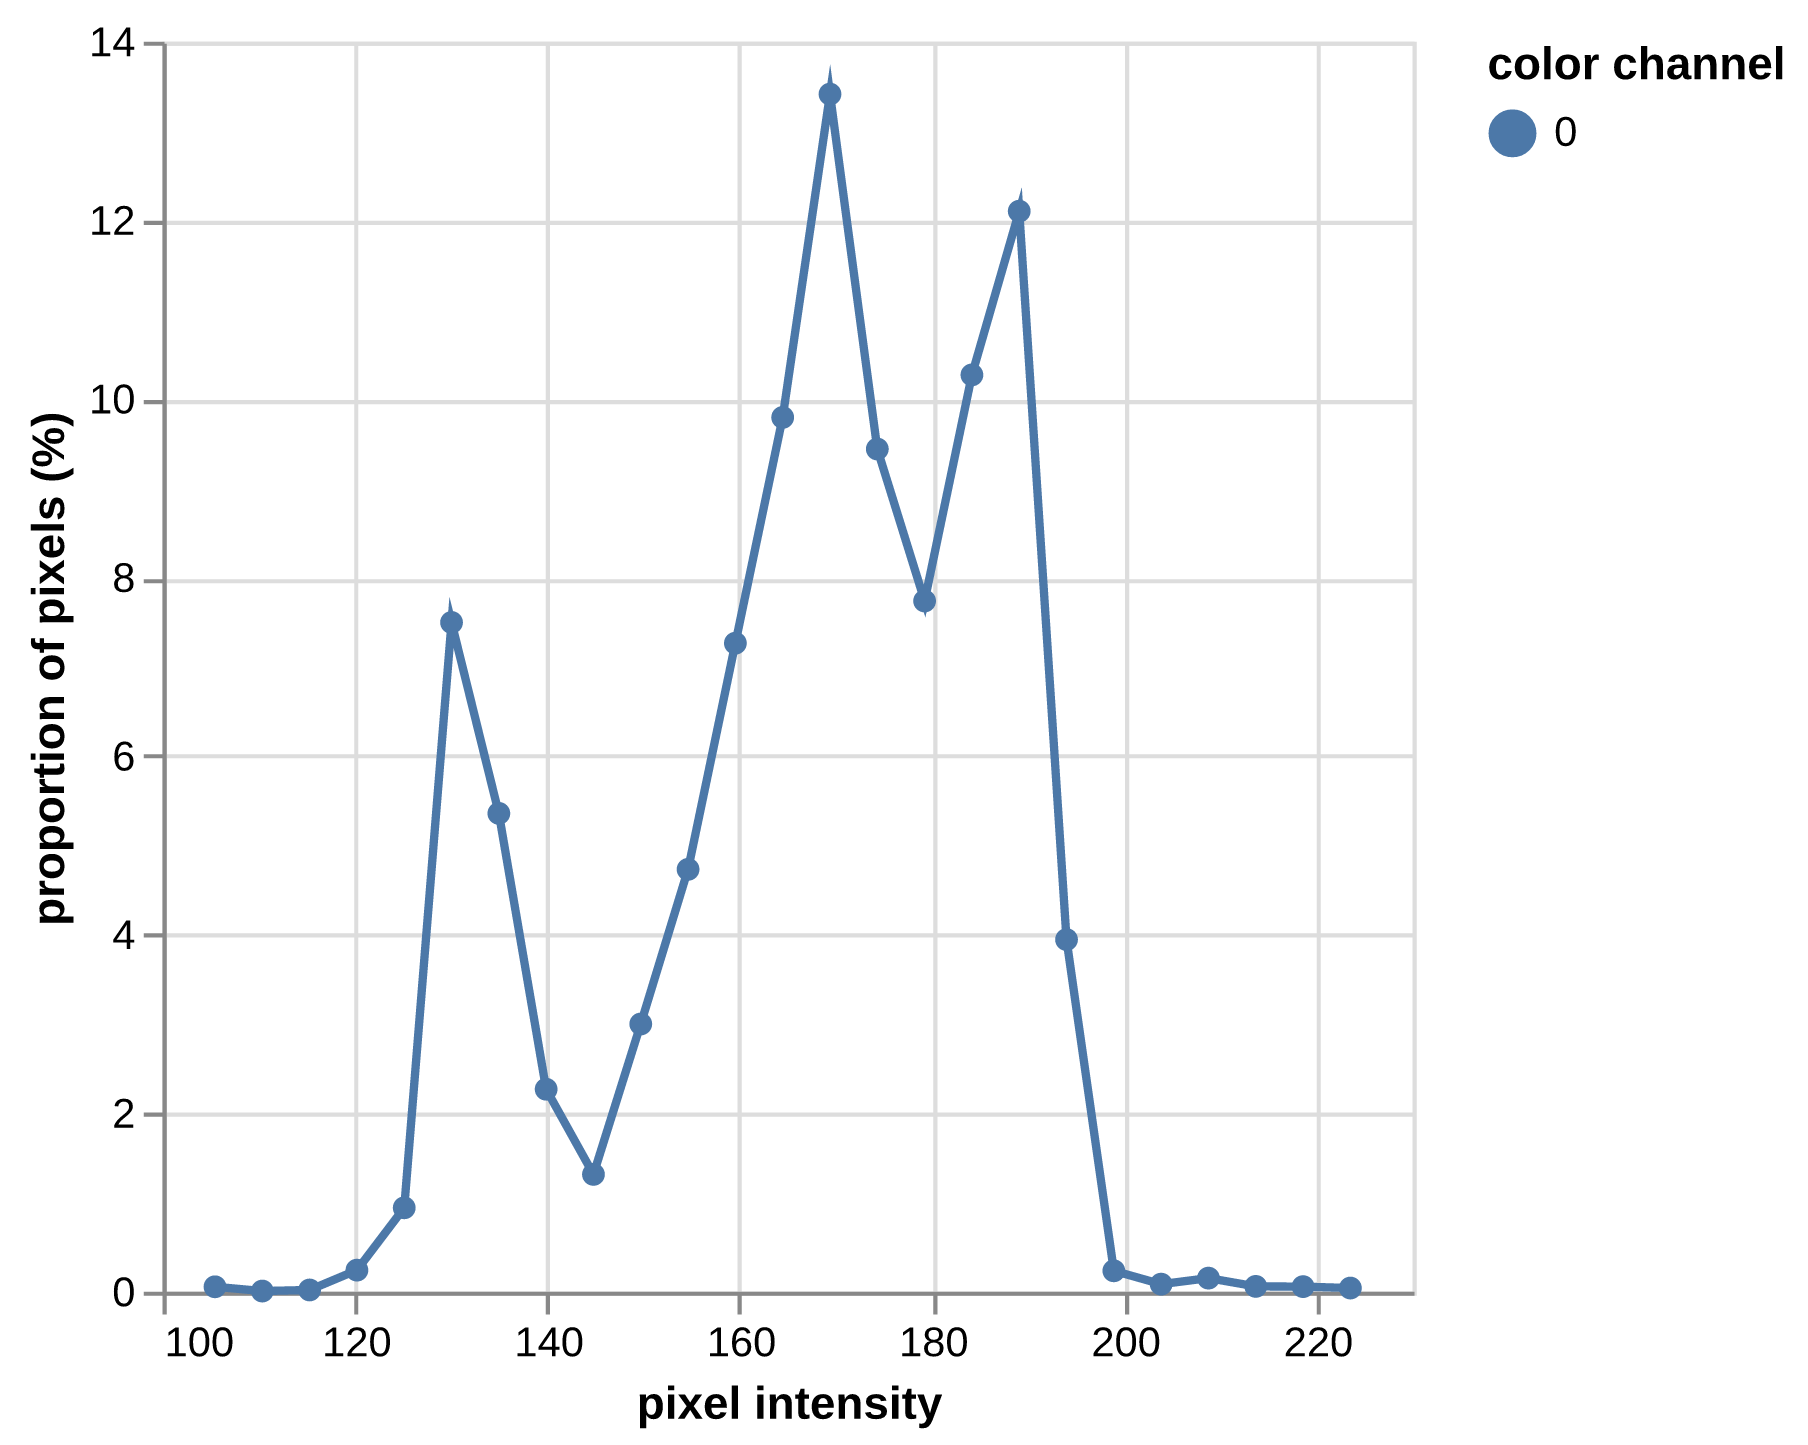
\includegraphics[width=0.5\textwidth]{images/threshold_histogram.png}
    \caption{
    Example intensity histogram for a selected color channel. Ideally, plant
    pixels and background pixels form separate peaks. The threshold should be
    placed in the valley between these groups.
    }%
    \label{fig:threshold-histogram}
\end{figure}

Threshold values can be adjusted with \verb|--threshold VALUE|. After changing
the threshold, inspect the binary threshold debug image. Consult
\autoref{fig:threshold-comparison} for dialing in the setting. 

\begin{figure}[ht]
    \centering
    \begin{subfigure}{0.32\textwidth}
        \centering
        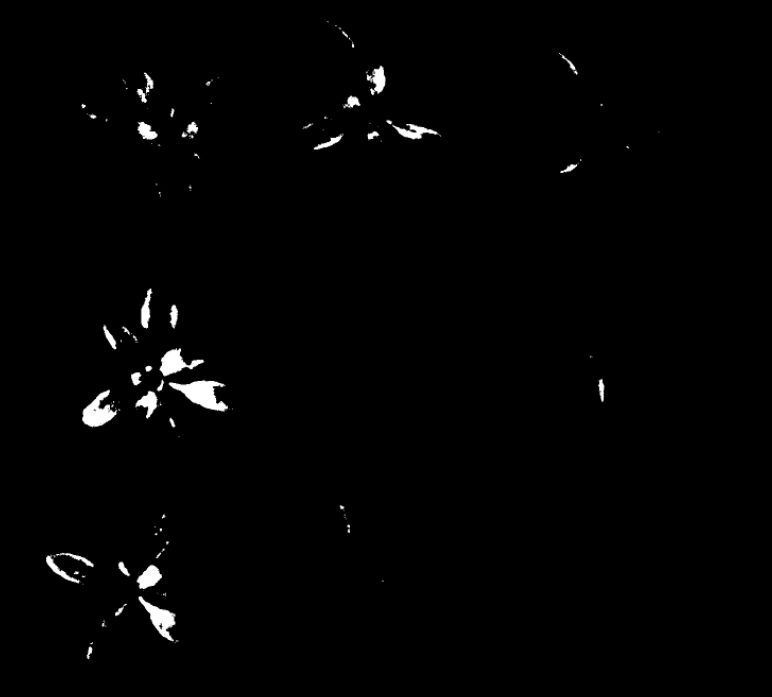
\includegraphics[width=\textwidth,height=4.8cm,keepaspectratio]{images/threshold_low.png}
        \caption{Threshold too low}
    \end{subfigure}
    \hspace{0.005\textwidth}
    \begin{subfigure}{0.32\textwidth}
        \centering
        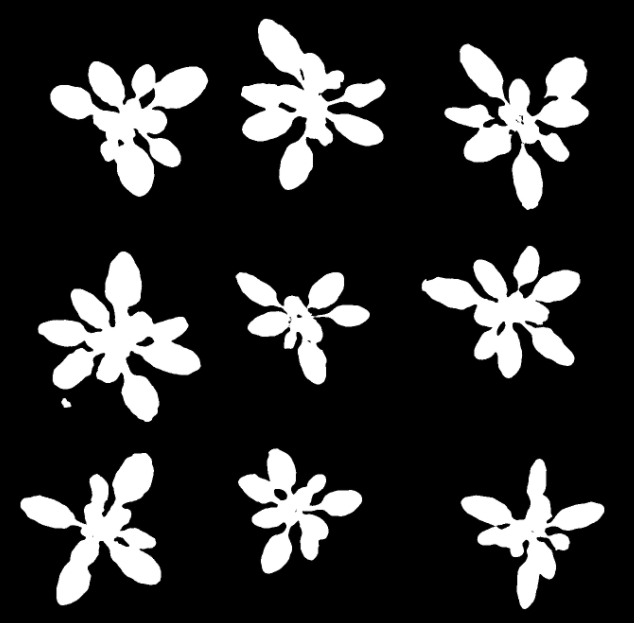
\includegraphics[width=\textwidth,height=4.8cm,keepaspectratio]{images/threshold_good.png}
        \caption{Threshold suitable}
    \end{subfigure}
    \hspace{0.005\textwidth}
    \begin{subfigure}{0.32\textwidth}
        \centering
        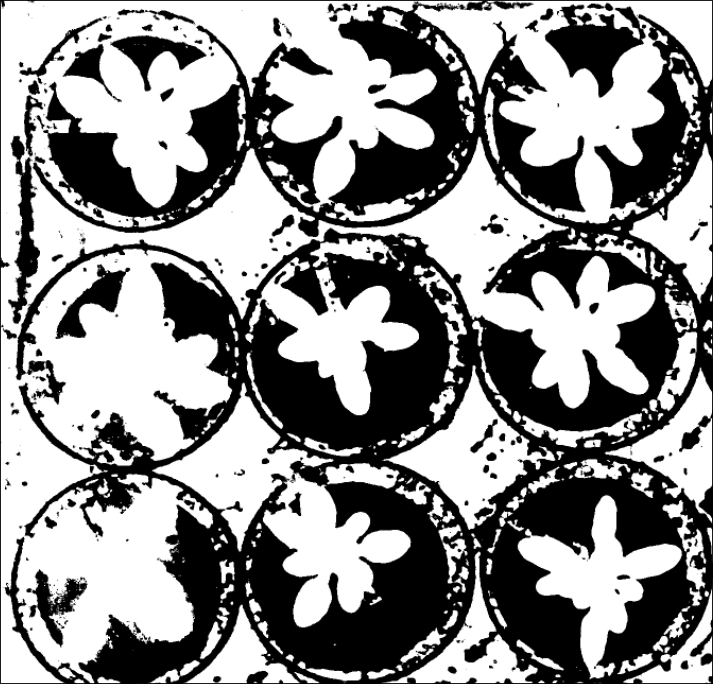
\includegraphics[width=\textwidth,height=4.8cm,keepaspectratio]{images/threshold_high.png}
        \caption{Threshold too high}
    \end{subfigure}
    \caption{
      Effect of different threshold values on the generated binary plant mask.
      Correct settings retain leaves while excluding non-plant objects.
    }%
    \label{fig:threshold-comparison}
\end{figure}

\subsection{Removing Noise with Fill Size}

After thresholding, small isolated artefacts often remain in the binary mask.
These are usually caused by reflections, algae, soil particles, or image noise.
The parameter \verb|--fill-size VALUE| removes objects smaller than a specified
number of pixels. Small values preserve more image detail but may retain noise
(\autoref{fig:fill-comparison}). Larger values remove more unwanted objects but
may also remove small plants or leaves. The fill-size parameter should
therefore be tuned using early time points, where plants are smallest.

\begin{figure}[ht]
    \centering
    \begin{subfigure}{0.32\textwidth}
        \centering
        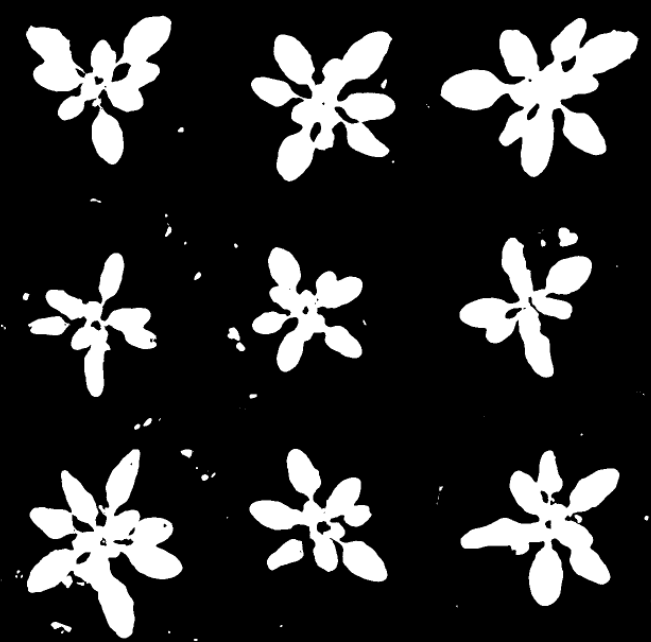
\includegraphics[width=\textwidth,height=4.8cm,keepaspectratio]{images/fill_low.png}
        \caption{Fill size too small}
    \end{subfigure}
    \hspace{0.005\textwidth}
    \begin{subfigure}{0.32\textwidth}
        \centering
        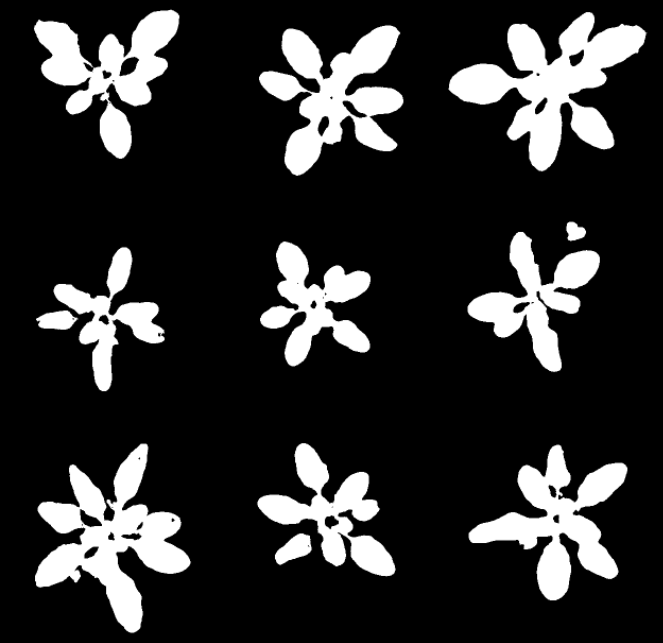
\includegraphics[width=\textwidth,height=4.8cm,keepaspectratio]{images/fill_good.png}
        \caption{Suitable fill size}
    \end{subfigure}
    \hspace{0.005\textwidth}
    \begin{subfigure}{0.32\textwidth}
        \centering
        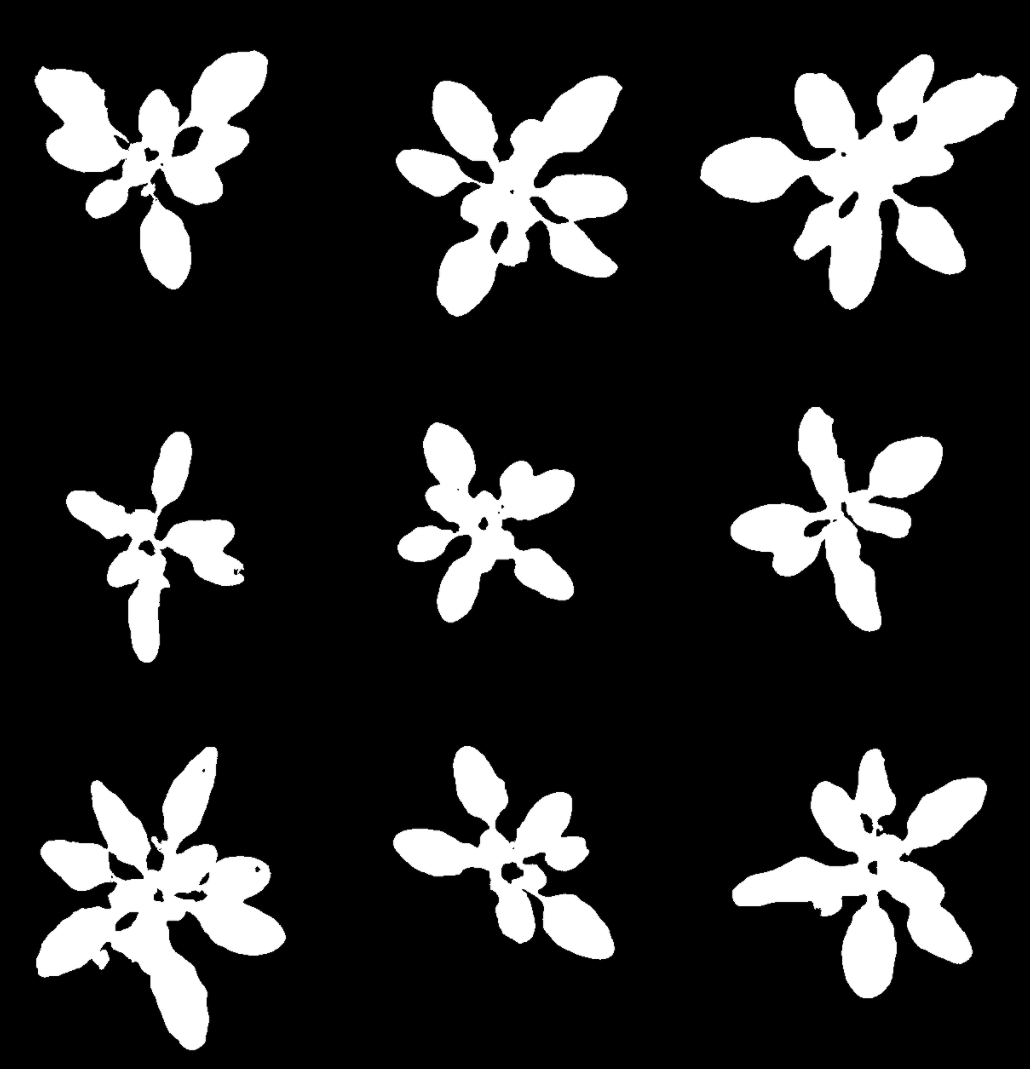
\includegraphics[width=\textwidth,height=4.8cm,keepaspectratio]{images/fill_high.png}
        \caption{Fill size too large}
    \end{subfigure}
    \caption{
      Effect of different fill-size settings. The optimal value removes
      background noise while preserving complete plant structures. Notice the
      missing leaves in C, which have been removed by a too aggressive fill.
    }%
    \label{fig:fill-comparison}
\end{figure}

\subsection{Regions of Interest}

Phenopi analyses plants within predefined regions of interest. Each region of
interest corresponds to one expected plant position in the tray
\autoref{fig:roi-grid-diagnostic}. The region-of-interest step is important
because it prevents neighbouring plants, tray edges, labels, colour cards, and
background areas from being included in the trait measurements. While Phenopi
has automatic ROI detection, manual specification is advised for optimal
results. The canopy analysis command can be run with an explicitly selected
rectangular analysis region. This rectangle is defined by a width
(\verb|--grid-width|), height (\verb|--grid-width|), and coordinates of its
top-left corner (\verb|--grid-x| and \verb|--grid-y|). This region should
contain all pots that need to be analysed, while excluding as much irrelevant
background as possible.

Next, Phenopi needs to know about the expected tray layout. These can be
specified with \verb|--rows| and \verb|--columns|. The analysis region is then
subdivided into this regular grid, and each cell is treated as the region of
interest for one plant. 

\begin{figure}[ht]
    \centering
    \includegraphics[width=0.8\textwidth]{images/roi_overlay}
    \caption{
        Example ROI diagnostic image. Each generated region should correspond
        to one plant position. If the grid is shifted, rotated, or does not
        cover the full tray, the rectangle selection should be adjusted and the
        analysis rerun.
    }%
    \label{fig:roi-grid-diagnostic}
\end{figure}

The ROI debug image should always be inspected before using the extracted trait
table. If plants are missing from the results, or if measurements appear to be
assigned to the wrong plant, the ROI selection should be checked first. Common
causes of ROI problems include selecting a rectangle that is too small,
selecting a rectangle that includes too much background, using the wrong number
of rows or columns, or analysing images where the tray shifted relative to the
selected rectangle.

\subsection{Checking Analysis Quality}

A good segmentation should include all visible leaf tissue while excluding
background material. Users should inspect images from the beginning, middle,
and end of the experiment. Small random errors are usually acceptable.
Systematic errors are more problematic because they may create artificial
growth patterns. Examples include gradually increasing algae detection,
changing shadows, unstable lighting or a moved plant tray. If technical
replicate images were collected, measurements from replicate captures should be
similar. Large differences between replicate images may indicate unstable
lighting conditions or poor segmentation settings.
